% !TeX program = xelatex
\documentclass{article}
\usepackage{kotex}
\usepackage[a4paper,left=3cm, right=3cm, top=2cm, bottom=2cm]{geometry}
\usepackage{amsmath}
\usepackage{graphicx}
\usepackage{caption}
\usepackage{setspace}
\usepackage{xcolor}
\usepackage{titlesec}
\usepackage{amssymb}
\usepackage{tcolorbox}
\usepackage{wrapfig}
\usepackage{amsthm}
\usepackage{multirow}
\usepackage{array}
\usepackage{tikz}
\usepackage{longtable}
\usepackage{pgfplots}
\pgfplotsset{compat=1.18}

\title{1.1 Introduction to Systems of Linear Equations}
\date{}
\author{}
\setstretch{1.3}

\titleformat{name=\section, numberless}
  {\normalfont\large\bfseries\color{blue}}
  {}
  {0pt}
  {}
\geometry{a4paper, margin=1in}

% Red subheading style (matches the textbook's red section headers)
\newcommand{\redheading}[1]{{\vspace{2mm}\noindent\Large\bfseries\color{red!55!black} #1\par}\vspace{2mm}}

\newtheoremstyle{mystyle}
  {}{}{\itshape}{}{\bfseries}{.}{.5em}{}
\theoremstyle{mystyle}

% Macro for the pseudo-3D "plane" parallelograms used in Figure 1.1.2
\newcommand{\planeA}[3]{
\begin{scope}[shift={(#1,#2)},rotate=#3]
\fill[cyan!12,draw=black,thick] (-1,-0.55) -- (1,-0.55) -- (1.3,0.55) -- (-0.7,0.55) -- cycle;
\end{scope}}

\begin{document}
\maketitle

\begin{tcolorbox}[colback=blue!5, colframe=blue!60!black, title=CHAPTER 1 OVERVIEW -- Systems of Linear Equations and Matrices, boxrule=0.5mm, arc=3mm]
Information in science, business, and mathematics is often organized into rows and columns to form rectangular arrays called ``matrices'' (plural of ``matrix''). Matrices often appear as tables of numerical data that arise from physical observations, but they occur in various mathematical contexts as well. For example, all of the information required to solve a system of equations such as
\[
5x+y=3,\qquad 2x-y=4
\]
is embodied in the matrix
\(
\begin{bmatrix} 5 & 1 & 3\\ 2 & -1 & 4\end{bmatrix}
\)
and the solution of the system can be obtained by performing appropriate operations on this matrix. It is the study of matrices and related topics that forms the mathematical field that we call \textbf{linear algebra}. In this chapter we will begin our study of matrices.
\end{tcolorbox}

\redheading{1.1 Introduction to Systems of Linear Equations}

{\itshape\color{blue!45!black}
Systems of linear equations and their solutions constitute one of the major topics that we will study in this course. In this first section we will introduce some basic terminology and discuss a method for solving such systems.\par}

\subsection*{Linear Equations}

\begin{tcolorbox}[
    colback=teal!4,
    colframe=teal!65!black,
    title=Definition \& Key Rules,
    fonttitle=\bfseries,
    boxrule=0.5mm,
    arc=3mm
    ]
    \textbf{\textcolor{teal!65!black}{Definition (Linear Equation).}}\quad
    A \textbf{linear equation} in the $n$ variables $x_1,x_2,\dots,x_n$ is one that can be expressed in the form
    \[
    a_1x_1+a_2x_2+\cdots+a_nx_n=b \tag{1}
    \]
    where $a_1,a_2,\dots,a_n$ and $b$ are constants, and the $a$'s are not all zero. In the special cases where $n=2$ or $n=3$, we will often use variables without subscripts and write linear equations as
    \[
    a_1x+a_2y=b,\qquad a_1x+a_2y+a_3z=b
    \]
    In the special case where $b=0$, Equation (1) has the form
    \[
    a_1x_1+a_2x_2+\cdots+a_nx_n=0
    \]
    which is called a \textbf{homogeneous linear equation} in the variables $x_1,x_2,\dots,x_n$.

    \noindent\textcolor{teal!50!black}{\rule{\linewidth}{0.4pt}}

    \textbf{\textcolor{teal!65!black}{Definition (System and Solution).}}\quad
    A finite set of linear equations is called a \textbf{system of linear equations} or, more briefly, a \textbf{linear system}. The variables are called \textbf{unknowns}. A \textbf{solution} of a linear system in $n$ unknowns $x_1,x_2,\dots,x_n$ is a sequence of $n$ numbers $s_1,s_2,\dots,s_n$ for which the substitution $x_1=s_1,\dots,x_n=s_n$ makes each equation a true statement. Such a solution can be written as
    \[
    (s_1,s_2,\dots,s_n)
    \]
    which is called an \textbf{ordered $n$-tuple}. If $n=2$, then the $n$-tuple is called an \textbf{ordered pair}, and if $n=3$, then it is called an \textbf{ordered triple}.
\end{tcolorbox}

\subsection*{EXAMPLE 1 | Linear Equations}
Observe that a linear equation does not involve any products or roots of variables. All variables occur only to the first power and do not appear, for example, as arguments of trigonometric, logarithmic, or exponential functions. The following are linear equations:
\[
x+3y=7,\qquad x_1-2x_2-3x_3+x_4=0,\qquad \tfrac12 x-y+3z=-1,\qquad x_1+x_2+\cdots+x_n=1
\]
The following are \emph{not} linear equations:
\[
x+3y^2=4,\qquad 3x+2y-xy=5,\qquad \sin x+y=0,\qquad \sqrt{x_1}+2x_2+x_3=1
\]

\redheading{Linear Systems in Two and Three Unknowns}

Linear systems in two unknowns arise in connection with intersections of lines. Consider the linear system
\[
a_1x+b_1y=c_1,\qquad a_2x+b_2y=c_2
\]
in which the graphs of the equations are lines in the $xy$-plane. Each solution $(x,y)$ of this system corresponds to a point of intersection of the lines, so there are three possibilities (\textbf{Figure 1.1.1}):
\begin{enumerate}
    \item The lines may be parallel and distinct, in which case there is no intersection and consequently no solution.
    \item The lines may intersect at only one point, in which case the system has exactly one solution.
    \item The lines may coincide, in which case there are infinitely many points of intersection (the points on the common line) and consequently infinitely many solutions.
\end{enumerate}

\begin{figure}[h]
\centering
\begin{tabular}{ccc}
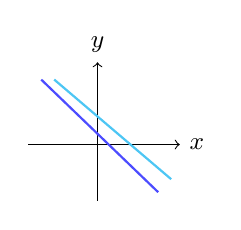
\begin{tikzpicture}[scale=0.55]
 \draw[->] (-1.6,0)--(1.9,0) node[right]{\small$x$};
 \draw[->] (0,-1.3)--(0,1.9) node[above]{\small$y$};
 \draw[blue!70,thick] (-1.3,1.5)--(1.4,-1.1);
 \draw[cyan!70,thick] (-1.0,1.5)--(1.7,-0.8);
\end{tikzpicture}
&
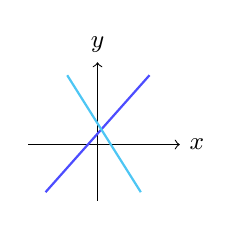
\begin{tikzpicture}[scale=0.55]
 \draw[->] (-1.6,0)--(1.9,0) node[right]{\small$x$};
 \draw[->] (0,-1.3)--(0,1.9) node[above]{\small$y$};
 \draw[blue!70,thick] (-1.2,-1.1)--(1.2,1.6);
 \draw[cyan!70,thick] (-0.7,1.6)--(1.0,-1.1);
\end{tikzpicture}
&
\begin{tikzpicture}[scale=0.55]
 \draw[->] (-1.6,0)--(1.9,0) node[right]{\small$x$};
 \draw[->] (0,-1.3)--(0,1.9) node[above]{\small$y$};
 \draw[blue!70,thick] (-1.2,-0.9)--(1.4,1.6);
 \draw[cyan!70,thick,dashed] (-1.2,-0.9)--(1.4,1.6);
\end{tikzpicture}
\\[1mm]
\fbox{\small No solution} & \fbox{\small One solution} & \fbox{\small \begin{tabular}{c}Infinitely many solutions\\(coincident lines)\end{tabular}}
\end{tabular}
\caption*{\textbf{FIGURE 1.1.1}}
\end{figure}

In general, we say that a linear system is \textbf{consistent} if it has at least one solution and \textbf{inconsistent} if it has no solutions. Thus, a consistent linear system of two equations in two unknowns has either one solution or infinitely many solutions---there are no other possibilities. The same is true for a linear system of three equations in three unknowns
\[
a_1x+b_1y+c_1z=d_1,\quad a_2x+b_2y+c_2z=d_2,\quad a_3x+b_3y+c_3z=d_3
\]
in which the graphs of the equations are planes. The solutions of the system, if any, correspond to points where all three planes intersect, so again we see that there are only three possibilities---no solutions, one solution, or infinitely many solutions (\textbf{Figure 1.1.2}).

\begin{figure}[h]
\centering
\begin{tabular}{cccc}
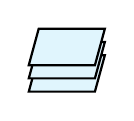
\begin{tikzpicture}[scale=0.42]
\planeA{0}{-0.4}{0}\planeA{0}{0}{0}\planeA{0}{0.4}{0}
\end{tikzpicture} &

\begin{tikzpicture}[scale=0.42]
\planeA{0}{-0.3}{0}\planeA{0}{0.3}{0}\planeA{0}{0}{35}
\end{tikzpicture} &

\begin{tikzpicture}[scale=0.42]
\planeA{-0.3}{0}{0}\planeA{0.3}{0.2}{60}\planeA{0}{-0.3}{-60}
\end{tikzpicture} &
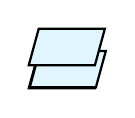
\begin{tikzpicture}[scale=0.42]
\planeA{0}{0}{0}\planeA{0.03}{0.03}{0}\planeA{0}{0.7}{0}
\end{tikzpicture}
\\
\fbox{\scriptsize \begin{tabular}{c}No solutions\\(three parallel planes)\end{tabular}} &
\fbox{\scriptsize \begin{tabular}{c}No solutions\\(two parallel planes)\end{tabular}} &
\fbox{\scriptsize \begin{tabular}{c}No solutions\\(no common intersection)\end{tabular}} &
\fbox{\scriptsize \begin{tabular}{c}No solutions (two coincident\\planes parallel to the third)\end{tabular}}
\\[2mm]

\begin{tikzpicture}[scale=0.42]
\planeA{-0.3}{0.15}{15}\planeA{0.3}{0.15}{-15}\planeA{0}{-0.35}{0}
\end{tikzpicture} &

\begin{tikzpicture}[scale=0.42]
\planeA{0}{0}{-25}\planeA{0}{0}{0}\planeA{0}{0}{25}
\end{tikzpicture} &
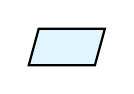
\begin{tikzpicture}[scale=0.42]
\planeA{0}{0}{0}
\end{tikzpicture} &

\begin{tikzpicture}[scale=0.42]
\planeA{0}{0}{0}\planeA{0.03}{0.03}{0}\planeA{0}{0}{30}
\end{tikzpicture}
\\
\fbox{\scriptsize \begin{tabular}{c}One solution\\(intersection is a point)\end{tabular}} &
\fbox{\scriptsize \begin{tabular}{c}Infinitely many solutions\\(intersection is a line)\end{tabular}} &
\fbox{\scriptsize \begin{tabular}{c}Infinitely many solutions\\(planes all coincident)\end{tabular}} &
\fbox{\scriptsize \begin{tabular}{c}Infinitely many solutions (two\\coincident planes; intersection is a line)\end{tabular}}
\end{tabular}
\caption*{\textbf{FIGURE 1.1.2}}
\end{figure}

We will prove later that our observations about the number of solutions of linear systems of two equations in two unknowns and linear systems of three equations in three unknowns actually hold for \emph{all} linear systems. That is:

\begin{tcolorbox}[colback=red!4, colframe=red!60!black, title=Theorem, boxrule=0.5mm, arc=3mm]
Every system of linear equations has \textbf{zero, one, or infinitely many solutions}. There are no other possibilities.
\end{tcolorbox}

\subsection*{EXAMPLE 2 | A Linear System with One Solution}
Solve the linear system
\[
x-y=1,\qquad 2x+y=6
\]
\textbf{SOLUTION:} We can eliminate $x$ from the second equation by adding $-2$ times the first equation to the second. This yields the simplified system
\[
x-y=1,\qquad 3y=4
\]
From the second equation we obtain $y=\tfrac43$, and on substituting this value in the first equation we obtain $x=1+y=\tfrac73$. Thus, the system has the unique solution
\[
x=\tfrac73,\quad y=\tfrac43
\]
Geometrically, this means that the lines represented by the equations in the system intersect at the single point $\left(\tfrac73,\tfrac43\right)$.

\subsection*{EXAMPLE 3 | A Linear System with No Solutions}
Solve the linear system
\[
x+y=4,\qquad 3x+3y=6
\]
\textbf{SOLUTION:} We can eliminate $x$ from the second equation by adding $-3$ times the first equation to the second equation. This yields the simplified system
\[
x+y=4,\qquad 0=-6
\]
The second equation is contradictory, so the given system has no solution. Geometrically, this means that the lines corresponding to the equations in the original system are parallel and distinct.

\subsection*{EXAMPLE 4 | A Linear System with Infinitely Many Solutions}
Solve the linear system
\[
4x-2y=1,\qquad 16x-8y=4
\]
\textbf{SOLUTION:} We can eliminate $x$ from the second equation by adding $-4$ times the first equation to the second. This yields the simplified system
\[
4x-2y=1,\qquad 0=0
\]
The second equation does not impose any restrictions on $x$ and $y$ and hence can be omitted. Thus, the solutions of the system are those values of $x$ and $y$ that satisfy the single equation
\[
4x-2y=1 \tag{8}
\]
Geometrically, this means the lines corresponding to the two equations in the original system coincide. Solving (8) for $x$ in terms of $y$, we obtain $x=\tfrac14+\tfrac12y$, and then assigning an arbitrary value $t$ (a \textbf{parameter}) to $y$, we can express the solution by the \textbf{parametric equations}
\[
x=\tfrac14+\tfrac12t,\qquad y=t
\]
For example, $t=0,1,-1$ yield the solutions $\left(\tfrac14,0\right),\left(\tfrac34,1\right),\left(-\tfrac14,-1\right)$.

\subsection*{EXAMPLE 5 | A Linear System with Infinitely Many Solutions}
Solve the linear system
\[
x-y+2z=5,\qquad 2x-2y+4z=10,\qquad 3x-3y+6z=15
\]
\textbf{SOLUTION:} This system can be solved by inspection, since the second and third equations are multiples of the first. Geometrically, this means that the three planes coincide and that those values of $x$, $y$, and $z$ that satisfy the equation
\[
x-y+2z=5 \tag{9}
\]
automatically satisfy all three equations. Thus, it suffices to find the solutions of (9). Solving this equation for $x$ in terms of $y$ and $z$, then assigning arbitrary values $r$ and $s$ (parameters) to these two variables, we obtain the parametric equations
\[
x=5+r-2s,\qquad y=r,\qquad z=s
\]
For example, taking $r=1$ and $s=0$ yields the solution $(6,1,0)$.

\redheading{Augmented Matrices and Elementary Row Operations}

As the number of equations and unknowns in a linear system increases, so does the complexity of the algebra involved in finding solutions. The required computations can be made more manageable by simplifying notation and standardizing procedures.

\begin{tcolorbox}[
    colback=teal!4,
    colframe=teal!65!black,
    title=Definition \& Key Rules,
    fonttitle=\bfseries,
    boxrule=0.5mm,
    arc=3mm
    ]
    \textbf{\textcolor{teal!65!black}{Definition (Augmented Matrix).}}\quad
    For the linear system
    \[
    \begin{aligned}
    a_{11}x_1+a_{12}x_2+\cdots+a_{1n}x_n&=b_1\\
    a_{21}x_1+a_{22}x_2+\cdots+a_{2n}x_n&=b_2\\
    &\ \ \vdots\\
    a_{m1}x_1+a_{m2}x_2+\cdots+a_{mn}x_n&=b_m
    \end{aligned}
    \]
    the rectangular array
    \[
    \begin{bmatrix}
    a_{11}&a_{12}&\cdots&a_{1n}&b_1\\
    a_{21}&a_{22}&\cdots&a_{2n}&b_2\\
    \vdots&\vdots&&\vdots&\vdots\\
    a_{m1}&a_{m2}&\cdots&a_{mn}&b_m
    \end{bmatrix}
    \]
    is called the \textbf{augmented matrix} for the system.

    \noindent\textcolor{teal!50!black}{\rule{\linewidth}{0.4pt}}

    \textbf{\textcolor{teal!65!black}{Key Rule (Elementary Row Operations).}}\quad
    The basic method for solving a linear system is to perform algebraic operations on the system that do not alter the solution set:
    \begin{enumerate}
        \item Multiply an equation (row) through by a nonzero constant.
        \item Interchange two equations (rows).
        \item Add a constant times one equation (row) to another.
    \end{enumerate}
    These three operations performed on the rows of an augmented matrix are called \textbf{elementary row operations}.
\end{tcolorbox}

\subsection*{EXAMPLE 6 | Using Elementary Row Operations}
In the left column we solve a system of linear equations by operating on the equations in the system, and in the right column we solve the same system by operating on the rows of the augmented matrix.

\begin{center}
\renewcommand{\arraystretch}{1.6}
\begin{longtable}{|p{7cm}|p{7cm}|}
\hline
\multicolumn{2}{|l|}{\textbf{Initial linear system}} \\
\hline
\(\begin{aligned} x+\ y+2z&=9\\ 2x+4y-3z&=1\\ 3x+6y-5z&=0\end{aligned}\)
&
\(\begin{bmatrix} 1&1&2&9\\ 2&4&-3&1\\ 3&6&-5&0\end{bmatrix}\)
\\
\hline
\multicolumn{2}{|l|}{Add $-2$ times the first equation/row to the second to obtain} \\
\hline
\(\begin{aligned} x+y+2z&=9\\ 2y-7z&=-17\\ 3x+6y-5z&=0\end{aligned}\)
&
\(\begin{bmatrix} 1&1&2&9\\ 0&2&-7&-17\\ 3&6&-5&0\end{bmatrix}\)
\\
\hline
\multicolumn{2}{|l|}{Add $-3$ times the first equation/row to the third to obtain} \\
\hline
\(\begin{aligned} x+y+2z&=9\\ 2y-7z&=-17\\ 3y-11z&=-27\end{aligned}\)
&
\(\begin{bmatrix} 1&1&2&9\\ 0&2&-7&-17\\ 0&3&-11&-27\end{bmatrix}\)
\\
\hline
\multicolumn{2}{|l|}{Multiply the second equation/row by $\tfrac12$ to obtain} \\
\hline
\(\begin{aligned} x+y+2z&=9\\ y-\tfrac72 z&=-\tfrac{17}2\\ 3y-11z&=-27\end{aligned}\)
&
\(\begin{bmatrix} 1&1&2&9\\ 0&1&-\tfrac72&-\tfrac{17}2\\ 0&3&-11&-27\end{bmatrix}\)
\\
\hline
\multicolumn{2}{|l|}{Add $-3$ times the second equation/row to the third to obtain} \\
\hline
\(\begin{aligned} x+y+2z&=9\\ y-\tfrac72 z&=-\tfrac{17}2\\ -\tfrac12 z&=-\tfrac32\end{aligned}\)
&
\(\begin{bmatrix} 1&1&2&9\\ 0&1&-\tfrac72&-\tfrac{17}2\\ 0&0&-\tfrac12&-\tfrac32\end{bmatrix}\)
\\
\hline
\multicolumn{2}{|l|}{Multiply the third equation/row by $-2$ to obtain} \\
\hline
\(\begin{aligned} x+y+2z&=9\\ y-\tfrac72 z&=-\tfrac{17}2\\ z&=3\end{aligned}\)
&
\(\begin{bmatrix} 1&1&2&9\\ 0&1&-\tfrac72&-\tfrac{17}2\\ 0&0&1&3\end{bmatrix}\)
\\
\hline
\multicolumn{2}{|l|}{Add $-1$ times the second equation/row to the first to obtain} \\
\hline
\(\begin{aligned} x+\tfrac{11}2 z&=\tfrac{35}2\\ y-\tfrac72 z&=-\tfrac{17}2\\ z&=3\end{aligned}\)
&
\(\begin{bmatrix} 1&0&\tfrac{11}2&\tfrac{35}2\\ 0&1&-\tfrac72&-\tfrac{17}2\\ 0&0&1&3\end{bmatrix}\)
\\
\hline
\multicolumn{2}{|l|}{Add $-\tfrac{11}2$ times the third equation/row to the first and $\tfrac72$ times the third to the second to obtain} \\
\hline
\(\begin{aligned} x&=1\\ y&=2\\ z&=3\end{aligned}\)
&
\(\begin{bmatrix} 1&0&0&1\\ 0&1&0&2\\ 0&0&1&3\end{bmatrix}\)
\\
\hline
\end{longtable}
\end{center}

\noindent The solution $x=1,\ y=2,\ z=3$ is now evident.

\section*{Exercise Set 1.1}
\begin{enumerate}
    \item[1.] In each part, determine whether the equation is linear in $x_1, x_2$, and $x_3$.\\
    (a) $x_1+5x_2-\sqrt2\,x_3=1$\quad (b) $x_1+3x_2+x_1x_3=2$\quad (c) $x_1=-7x_2+3x_3$\\
    (d) $x_1^{-2}+x_2+8x_3=5$\quad (e) $x_1^{3/5}-2x_2+x_3=4$\quad (f) $\pi x_1-\sqrt2\,x_2=7^{1/3}$

    \item[3.] Using the notation of Formula (7), write down a general linear system of\\
    (a) two equations in two unknowns.\quad (b) three equations in three unknowns.\quad (c) two equations in four unknowns.

    \item[5.] In each part, find a system of linear equations in the unknowns $x_1,x_2,x_3,\dots$ that corresponds to the given augmented matrix.\\
    (a) $\begin{bmatrix}2&0&0\\3&-4&0\\0&1&1\end{bmatrix}$\qquad
    (b) $\begin{bmatrix}3&0&-2&5\\7&1&4&-3\\0&-2&1&7\end{bmatrix}$

    \item[7.] Find the augmented matrix for each linear system.\\
    (a) $-2x_1=6,\ 3x_1=8,\ 9x_1=-3$\qquad
    (b) $6x_1-x_2+3x_3=4,\ 5x_2-x_3=1$\\
    (c) $2x_2-3x_4+x_5=0,\ -3x_1-x_2+x_3=-1,\ 6x_1+2x_2-x_3+2x_4-3x_5=6$

    \item[9.] In each part, determine whether the given 3-tuple is a solution of the linear system
    \[
    2x_1-4x_2-x_3=1,\quad x_1-3x_2+x_3=1,\quad 3x_1-5x_2-3x_3=1
    \]
    (a) $(3,1,1)$\quad (b) $(3,-1,1)$\quad (c) $(13,5,2)$\quad (d) $\left(\tfrac{13}2,\tfrac52,2\right)$\quad (e) $(17,7,5)$

    \item[11.] In each part, solve the linear system, if possible, and use the result to determine whether the lines represented by the equations in the system have zero, one, or infinitely many points of intersection. If there is a single point of intersection, give its coordinates, and if there are infinitely many, find parametric equations for them.\\
    (a) $3x-2y=4,\ 6x-4y=9$\qquad (b) $2x-4y=1,\ 4x-8y=2$\qquad (c) $x-2y=0,\ x-4y=8$

    \item[13.] Use parametric equations to describe the solution set of each linear equation.\\
    (a) $7x-5y=3$\quad (b) $3x_1-5x_2+4x_3=7$\quad (c) $-8x_1+2x_2-5x_3+6x_4=1$\quad (d) $3v-8w+2x-y+4z=0$

    \item[15.] Each of the following linear systems has infinitely many solutions. Use parametric equations to describe its solution set.\\
    (a) $2x-3y=1,\ 6x-9y=3$\qquad
    (b) $x_1+3x_2-x_3=-4,\ 3x_1+9x_2-3x_3=-12,\ -x_1-3x_2+x_3=4$

    \item[17.] Find a single elementary row operation that will create a 1 in the upper left corner of the given augmented matrix and will not create any fractions in its first row.\\
    (a) $\begin{bmatrix}-3&-1&2&4\\2&-3&3&2\\0&2&-3&1\end{bmatrix}$\qquad
    (b) $\begin{bmatrix}0&-1&-5&0\\2&-9&3&2\\1&4&-3&3\end{bmatrix}$

    \item[19.] Find all values of $k$ for which the given augmented matrix corresponds to a consistent linear system.\\
    (a) $\begin{bmatrix}1&k&-4\\4&8&2\end{bmatrix}$\qquad
    (b) $\begin{bmatrix}1&k&-1\\4&8&-4\end{bmatrix}$

    \item[21.] The curve $y=ax^2+bx+c$ shown in the accompanying figure passes through the points $(x_1,y_1),(x_2,y_2)$, and $(x_3,y_3)$. Show that the coefficients $a,b,c$ form a solution of the system of linear equations whose augmented matrix is
    \[
    \begin{bmatrix} x_1^2&x_1&1&y_1\\ x_2^2&x_2&1&y_2\\ x_3^2&x_3&1&y_3\end{bmatrix}
    \]
    \begin{figure}[h]
    \centering
    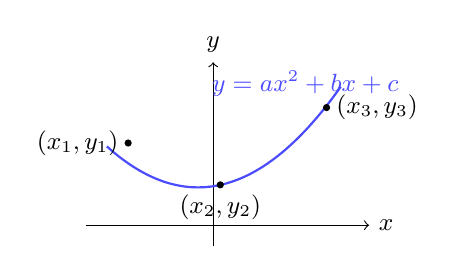
\begin{tikzpicture}[scale=0.9]
    \draw[->] (-1.8,0)--(2.2,0) node[right]{\small$x$};
    \draw[->] (0,-0.3)--(0,2.3) node[above]{\small$y$};
    \draw[blue!70,thick,domain=-1.5:1.8,samples=60] plot(\x,{0.35*\x*\x+0.15*\x+0.55});
    \filldraw[black] (-1.2,1.16) circle (1.2pt) node[left]{\small$(x_1,y_1)$};
    \filldraw[black] (0.1,0.57) circle (1.2pt) node[below]{\small$(x_2,y_2)$};
    \filldraw[black] (1.6,1.66) circle (1.2pt) node[right]{\small$(x_3,y_3)$};
    \node[blue!70] at (1.3,2.0) {\small$y=ax^2+bx+c$};
    \end{tikzpicture}
    \caption*{\textbf{FIGURE Ex-21}}
    \end{figure}

    \item[23.] Show that if the linear equations $x_1+kx_2=c$ and $x_1+lx_2=d$ have the same solution set, then the two equations are identical (i.e., $k=l$ and $c=d$).

    \item[25.] Suppose that a certain diet calls for 7 units of fat, 9 units of protein, and 16 units of carbohydrates for the main meal, and suppose that an individual has three possible foods to choose from to meet these requirements:\\
    Food 1: Each ounce contains 2 units of fat, 2 units of protein, and 4 units of carbohydrates.\\
    Food 2: Each ounce contains 3 units of fat, 1 unit of protein, and 2 units of carbohydrates.\\
    Food 3: Each ounce contains 1 unit of fat, 3 units of protein, and 5 units of carbohydrates.\\
    Let $x,y,z$ denote the number of ounces of the first, second, and third foods that the dieter will consume at the main meal. Find (but do not solve) a linear system in $x,y,z$ whose solution tells how many ounces of each food must be consumed to meet the diet requirements.

    \item[27.] Suppose you are asked to find three real numbers such that the sum of the numbers is 12, the sum of two times the first plus the second plus two times the third is 5, and the third number is one more than the first. Find (but do not solve) a linear system of equations whose solutions describe the three conditions.
\end{enumerate}

\end{document}
